\chapter{Analysis Of The Problem}\label{sec:chap:3}
Exercise is something that constitutes a major aspect of a person’s life from cross country running to weight training, and everything in between. The problem is that for many activities even though we now have access to massive amounts of information thanks to having access to the internet in the palm of our hands, it is still a pain to search for how to correctly exercise our bodies and what is best to efficiently do so. This makes something that improves our health to something that may cause injury.\\

 
This is reflected every year in gyms, where every New Year there is an influx of people that join and after a few weeks they end up abandoning their New Year’s resolution. In America 13 \% of all New Year’s resolutions are related to losing weight and exercising, making it the most common resolution. With google trends, that shows what users search for, we can corroborate these results with the interest people have of subjects like exercising and weight loss were there are major spikes of interest at the beginning of every year that slowly dies of towards the end of the year.\cite{newyear}


\begin{center}
	\begin{figure}[h!]
		\centering
		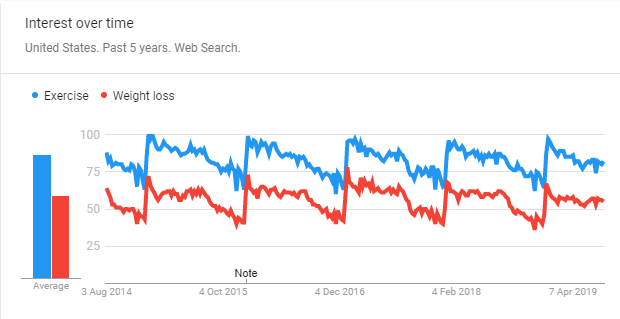
\includegraphics[scale=0.9]{./images/2-new-year-exercise}
		\caption{User Trends}
		\label{user-trends-gym}
	\end{figure}
\end{center}

Thanks to gym applications gaining popularity the amount of data gathered allows the creation of some interesting conclusions where in the following graph can be seen how many activity logs uploaded to Strava’s fitness app, this graph separates the different age groups which helps figure out which groups are more common to abandon and retake the gym after New Year. From the following graph older age groups have a higher tendency to start their resolutions as soon as possible, where younger age groups tend to have a smoother approach when starting their resolutions. What they have in common is that all groups show a decrease in activity logs towards the end of the year.\cite{newyear}\\

\begin{center}
	\begin{figure}[h!]
		\centering
		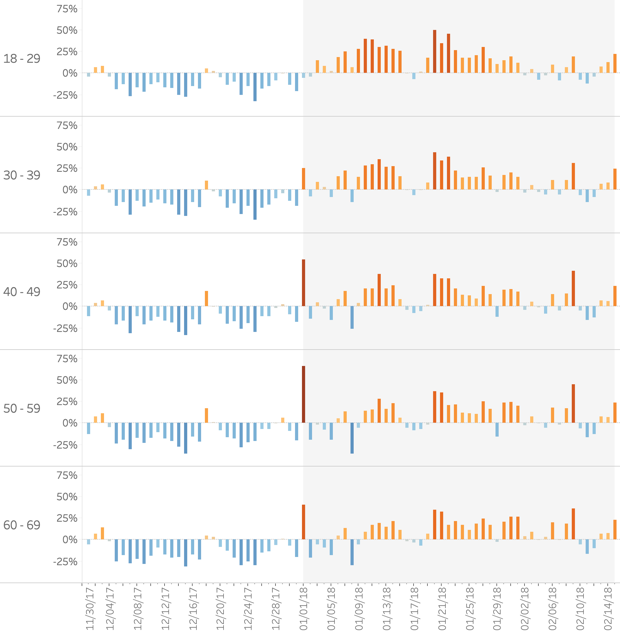
\includegraphics[scale=0.6]{./images/2-new-year-logs}
		\caption{User Activity Log Uploads}
		\label{user-logs-gym}
	\end{figure}
\end{center}

The conclusion of this analysis is that there is a motivation to get fit, but people have problems in maintaining their routines.  One of the reasons are unrealistic expectations where people want to tackle a big objective without being experienced or being disciplined, another of the reasons are boring workouts where people only do the exercises they have seen in films and don’t change their routine because they don’t have the knowledge to do so. Because of this and many other reasons the resolution to go to the gym quickly dies of.\cite{newyear_logs}\\

\section{Objectives}\label{sec:chap2_objectives}

The main objective is to have a functional virtual assistant that can provide the same help as normal personal trainers but at a much lower cost. This project will be a proof of concept with some limited functionality to see the viability of the product, the project will be focused on gym training.\\
The objective of the chatbot is to help users stay active, the way this will be accomplished is by making it easier for them to stay motivated and keep reaching their objectives. Reviewing the most common reasons people quit doing exercise comes down to unreasonable objectives and a lack of knowledge.\\

The following points reflect the main functionality the bot will have in it’s final form to help the user reach their goals:
\begin{itemize}
	\item {\textbf{Exercise table creation:}  One of the most time-consuming and boring things to do is prepare a routine to follow, there are applications that help out with this, but the idea for this project is to make the interaction more human-like, having the bot automatically generate tables based on what muscles have been trained and what muscles are not proportionate to the rest of the body. As this is a proof of concept and due to the time constraint of this project, the functionality that tracks what the user has exercised and the table creation will be limited.}
	\item {\textbf{Diets table creation:} Like what the above point talks about, the objective here is to make it easier for the user to know what to eat in order to reach their desired weight or to gain muscle mass. As some users may have different meal preferences, for the final product the chatbot can take food preferences in to account to provide different meals.}
	\item {\textbf{User tracking:} The objective is to track the user’s progress and see how close they are of fulfilling their goals, this will provide data on each user’s performance and how to further adapt their routines to make it easier to follow.}
	\item {\textbf{Motivate user regularly:} By checking how their training sessions are going and how well the users are progressing, motivate them with data on their progress and how close they are of achieving their goals.}
	\item {\textbf{Training sessions:} This objective would be an addition for future development as it requires a different architecture and it is still not technologically ready. The idea is to have a human-like voice speak while you complete your training sessions. The problem is making the voice human-like and the technology is not there yet. The idea of doing it written distracts the user by making the user use the phone more. }
	 
\end{itemize}	 
These objectives when completed will provide the user with enough tools to feel motivated and keep them using the application, where certain functionality may require being a premium member. This will fulfil the objective of making the application profitable, another way to increase profitability would be using ads related to health products the user can buy based on the chatbots recommendations, from protein shakes to measurement tools.















